\documentclass[aspectratio=169]{beamer}
\usepackage[utf8]{inputenc}
\usepackage[T1]{fontenc}
\usepackage{graphicx}
\usepackage{booktabs}
\usepackage{csquotes}
\usepackage{hyperref}
\usepackage{caption}
\usepackage{subcaption}
\usepackage{lipsum}
\usepackage{caption}

\usepackage[backend=biber,style=authoryear]{biblatex}
\usepackage{url}

\setbeamertemplate{navigation symbols}{}
\addbibresource{citations.bib}

\AtBeginSection[]{
    \begin{frame}[plain]
        \sectionpage
    \end{frame}
}

\usetheme{Madrid}
\usecolortheme{whale}
\setbeamertemplate{caption}[numbered]

\title[Integrating logical constraints in OCGNN for AD]{Integrating logical constraints \\in one-class graph neural networks for anomaly detection}
\subtitle{}
\author[A. Romanenko]{Anastasiia Romanenko}
\institute[TU Dortmund]{Technische Universität Dortmund \\ Fakultät Statistik}
\date[06.03.2026]{6. march 2026}



\begin{document}

\begin{frame}
  \titlepage
  \vspace{1cm}
  \centering
  \small
\end{frame}

\begin{frame}{Contents}
  \tableofcontents
\end{frame}

\section{Problem statement}

\begin{frame}{Importance of Anomaly Detection on Graph Data}
    An anomaly is an unusual or unexpected pattern in data. Detecting anomalies is important for identifying unknown threats and irregular behavior in complex systems.

    \begin{figure}[htpb]
        \centering
        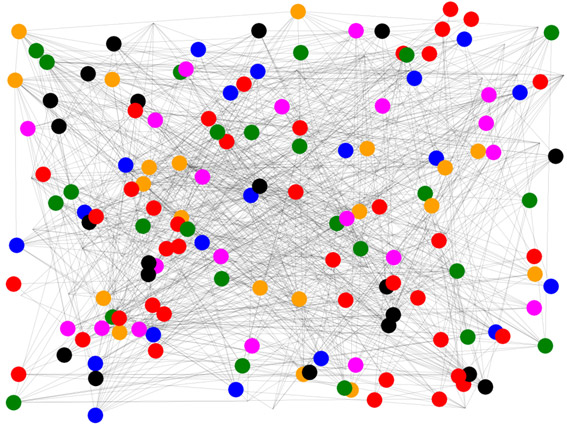
\includegraphics[width=7cm]{images/graph_picture.jpg}
        \label{fig:ocgin}
    \end{figure}
    
\end{frame}

\begin{frame}{Motivation of constraints driven graph AD}
    In many real-world application we have prior knowledge about data, which can be formulated as logical rules
    
    \begin{itemize}
        \item If $\texttt{person\_height} > 200\,\text{cm}$ $\rightarrow$ anomaly
        \item If a financial transaction graph contains a forbidden cycle pattern $\rightarrow$ anomaly
        \item If a molecular graph violates valence constraints $\rightarrow$ anomaly
    \end{itemize}
    \vspace{0.4cm}
    Classical One-Class Graph Neural Networks:
    \begin{itemize}
        \item learn only from data
        \item do not explicitly learn logical rules
        \item may learn representations that violate known knowledge
    \end{itemize}
\end{frame}

\section{Existing graph anomaly detection methods}

    \begin{frame}{Anomalies on graph data}
        \begin{figure}[htpb]
            \centering
            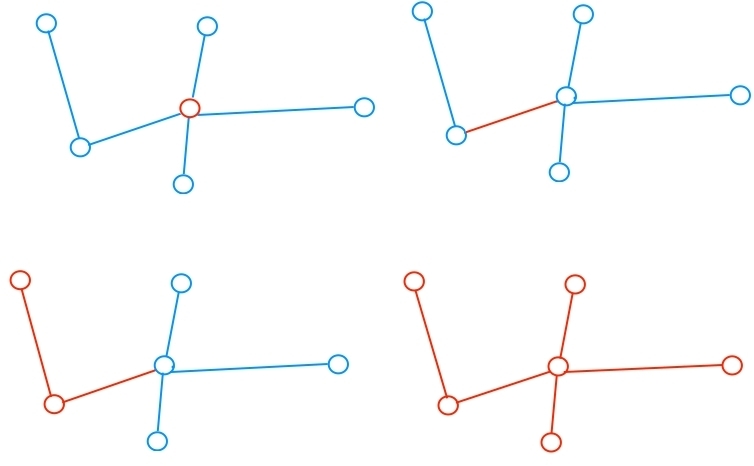
\includegraphics[width=10cm]{images/anomalies.jpg}
            \caption{Kinds of anomalies on graph data}
            \label{fig:scatter}
        \end{figure}
\end{frame}


\begin{frame}{Previous One-Class Graph Methods}
    Common assumptions:
    \begin{itemize}
        \item Access to a large set of normal graph data only
        \item Learn a graph embedding $f_\theta(G) \in \mathbb{R}^d$
        \item Model ``normality'' as a compact region in the embedding space
    \end{itemize}
    
    Typical objective (hypersphere learning):
    \[
    \min_{\theta} \sum_{i} 
    \left\| f_\theta(G_i) - c \right\|^2
    \]
    where $c$ denotes the center of normal data.
\end{frame}

\begin{frame}{OCGNN -- Structure}
    
    \begin{figure}[htpb]
        \centering
        
\includegraphics[width=15cm]{images/ocgin.pdf}
        \caption{Structure of OCGIN \footcite{ocgin}}
        \label{fig:ocgin}
    \end{figure}

\end{frame}

\begin{frame}{OCGNN -- Forward Pass}
    For a graph $G = (V, E)$ with node features $X \in \mathbb{R}^{|V| \times d_{in}}$:
    
    \[
    h_v^{(k+1)} = \text{MLP}^{(k)}\left( (1 + \epsilon) \cdot h_v^{(k)} + \sum_{u \in \mathcal{N}(v)} h_u^{(k)} \right)
    \]
    
    where $\epsilon$ is a learnable parameter, and the MLP consists of Linear $\rightarrow$ ReLU $\rightarrow$ Linear layers.
    
    \[
    z_i = \frac{1}{|V_i|} \sum_{v \in V_i} h_v^{(L)}
    \]
    Global mean pooling aggregates the node embeddings into a graph-level embedding $z_i \in \mathbb{R}^{d_{hidden}}$.
    
    \[
    L_{\text{OCGIN}} = \frac{1}{n} \sum_{i=1}^{n} \| z_i - c \|^2
    \]
    where $c$ is the center of normality (initialized as the mean of the normal data embeddings).
\end{frame}

\section{Existing Methods with Logical Constraints}

\begin{frame}{Existing Methods with Logical Constraints}
    
    \textbf{1) Constraints as Semantic Loss \footcite{xu2018semanticlossfunctiondeep}}
    \begin{itemize}
      \item Logical rules are manually encoded as differentiable loss terms
      \item The neural network is trained to minimize both the data loss and the constraint loss
    \end{itemize}

    \textbf{2) Fuzzy Logic in Loss \footcite{Badreddine_2022}}
    \begin{itemize}
      \item Logical rules are relaxed by applying continuous functions
    \end{itemize}
    
    \textbf{3) Constraint-aware Architectures \footcite{yang2023injectinglogicalconstraintsneural}}
    \begin{itemize}
      \item Logical rules compiled into network structure or output layer
      \item Guarantees or encourages valid structured outputs
    \end{itemize}
    
\end{frame}

\begin{frame}{Assumptions and Empirical Results}

    \textbf{Common Assumptions}
    \begin{itemize}
      \item Domain knowledge is available in the form of logical rules
      \item Constraints can be formulated as differentiable terms or probabilistically weighted
    \end{itemize}
    
    \textbf{Empirical Benefits}\footcite{Giunchiglia_2022}, 
    \footcite{stoian2024realisticsyntheticdataconstraining} 
    \begin{itemize}
      \item Improved performance
      \item Models are able to learn from less data 
      \item Increased interpretability through semantic rule satisfaction
    \end{itemize}

\end{frame}

\section{My approach}

\subsection{data}


\begin{frame}{Why Are Graph AD Datasets Uncommon?}
    \textbf{Problem with Collecting Graph AD Datasets:}
    \begin{itemize}
        \item Anomalies are rare, diverse, and unknown by definition (typically $< 5\%$ of the data)
        \item They are difficult to collect and label
    \end{itemize}
    
    \textbf{Common Solution: Pseudo-Labels}
    \begin{itemize}
        \item Use labeled graph datasets where one class is treated as normal
        \item Treat the majority class as ``normal'' and the minority class as ``anomaly''
    \end{itemize}
\end{frame}

\begin{frame}{My Approach: Logical Constraints}
    \textbf{Problem: Finding Logical Constraints}
    \begin{itemize}
        \item Domain knowledge is required to define rules for each dataset
        \item Domain experts are not always available
    \end{itemize}
    
    \textbf{Solution: Generate Constraints from Decision Trees}
    \begin{enumerate}
        \item Add graph-related features to the data (e.g., node degree)
        \item Train a decision tree on the (pseudo-)labeled data
        \item Extract logical rules from the decision tree paths
    \end{enumerate}
\end{frame}

\begin{frame}[fragile]{Example: Constraint JSON}
    \begin{small}
    \begin{verbatim}
{
  "constraints": [
    {
      "conditions": [
        {"feature_index": 1263, "op": "<=", "threshold": 0.0},
        {"feature_index": 205, "op": "<=", "threshold": 0.0}
      ],
      "predicted_class": 1,
      "meta": {"depth": 2, "y_label_number": "98 v.s. 243"}
    },
    ...
  ],
  "additional_attributes": {
    "0:1433": "node_features",
    "1433": "node_degree",
    "1434": "clustering_coefficient"
  }

    \end{verbatim}
    \end{small}
\end{frame}

\subsection{Implementing logical rules into OCGIN}

% TODO referenz
\begin{frame}{Hard Rules $\rightarrow$ differentiable fuzzy logic}
    \begin{columns}
        \column{0.6\textwidth}
        \begin{enumerate}
            \item \textbf{Feature Extraction:} Combine original features with derived features (e.g., node degree)
            \item \textbf{Rule Evaluation:} For each anomaly rule:
            \begin{itemize}
                \item Evaluate all conditions using soft logic
                \item Combine them with soft AND
            \end{itemize}
            \item \textbf{Combine Rules:} Apply soft OR over all rules
        \end{enumerate}
        
        \vspace{0.2cm}
        Output: A scalar violation score per node (higher values indicate stronger constraint violation for a chosen class of constraints)
        
        
        \column{0.4\textwidth}
        \textbf{Comparison operators:}
        \begin{itemize}
            \item $x \leq t \rightarrow \sigma(\lambda \cdot (t - x))$
            \item $x > t \rightarrow \sigma(\lambda \cdot (x - t))$
        \end{itemize}
        
        \textbf{Logic gates:}
        \begin{itemize}
            \item $A \land B \rightarrow \prod_i A_i$
            \item $A \lor B \rightarrow 1 - \prod_i (1 - A_i)$
        \end{itemize}
        
        
    \end{columns}
\end{frame}

\begin{frame}{Loss Functions in Node-Level OCGIN}
    Two variants have been implemented:
    
    \vspace{0.3cm}
    \textbf{Variant 1 -- Additive:}
    \[
    L_{\text{total}} = \frac{1}{n}\sum_{i=1}^{n} \|z_i - c\|^2 
    + \frac{1}{n}\sum_{i=1}^{n} L_{\text{cons}}(i)
    \]
    
    \textbf{Variant 2 -- Weighting:}
    \[
    L_{\text{total}} = \frac{1}{n}\sum_{i=1}^{n} 
    \left( \|z_i - c\|^2 * (1 + L_{\text{cons}}(i)) \right)
    \]

    \textbf{Variant 3 -- Ignoring suspicious nodes:}
    \[
    L_{\text{total}} = \frac{1}{n}\sum_{i=1}^{n} 
    \left( \|z_i - c\|^2 * (1 - L_{\text{cons}}(i)) \right)
    \]
    
    Here, $L_{\text{cons}}(i)$ denotes the soft rule violation for node $i$.
\end{frame}

\begin{frame}{Results of first experiments}
    \begin{figure}
        \centering
        
\includegraphics[width=\textwidth]{images/results_presentation.pdf}
    \end{figure}
\end{frame}


\begin{frame}{Future Work}
    \begin{itemize}
        \item Implement the already developed ``constraint score'' that indicates the predicted class based on the constraints and how much a node would need to change to switch its class
        \item Experiment with integrating soft logic in different ways: in the loss function, as a node or graph feature, or as an additional term in the message passing
        \item Evaluate the use of hard logical rules
        \item Apply the approach to OCGTL
    \end{itemize}
\end{frame}

\begin{frame}{}
    \centering
    \Large Thank you for your attention!
\end{frame}

\begin{frame}[allowframebreaks]{References}
\printbibliography
\end{frame}



\end{document}
